\documentclass[varwidth=true, border=2pt]{standalone}
\usepackage{tikz}
\usetikzlibrary{arrows,positioning, calc}
\tikzset{
    %Define standard arrow tip
    >=stealth',
    % Define arrow style
    pil/.style={->,thick}
}

\begin{document}
  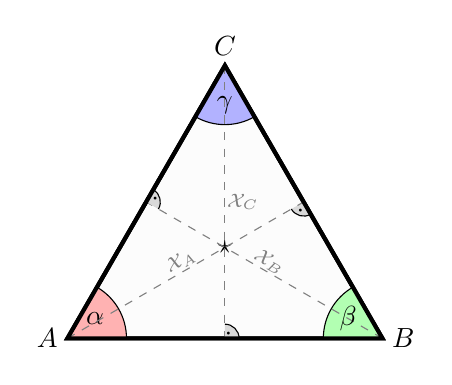
\begin{tikzpicture}
    % draw the background
    \draw [line width=1.5pt, fill=gray!2] (0,0) -- (60:4) -- (4,0) -- cycle;

    \coordinate[label=left:$A$]  (A) at (0,0);
    \coordinate[label=right:$B$] (B) at (4,0);
    \coordinate[label=above:$C$] (C) at (2,3.464);
    \coordinate[label=above:$\star$] (D) at (2,0.953);

%    \coordinate[label=below:$c$](c) at ($ (A)!.5!(B) $);
%    \coordinate[label=left:$b$](b) at ($ (A)!.5!(C) $);
%    \coordinate[label=right:$a$](a) at ($ (B)!.5!(C) $);

    % angle alpha
    \draw[fill=red!30] (0,0) -- (0:0.75cm) arc (0:60:.75cm);
    \draw (0.35cm,0.25cm) node {$\alpha$};

    % angle beta
    \begin{scope}[shift={(4cm,0cm)}]
        \draw[fill=green!30] (0,0) -- (-180:0.75cm) arc (180:120:0.75cm);
        \draw[color=gray, dashed] (0,0) -- node[sloped, above=-0.1cm] {$\scriptstyle \mathcal{X}_{B}$} (150:3.464cm);
        \draw (150:0.5cm) node {$\beta$};
    \end{scope}

    % angle gamma
    \begin{scope}[shift={(60:4)}]
        \draw[fill=blue!30] (0,0) -- (-120:.75cm) arc (-120:-60:.75cm);
        \draw[color=gray, dashed] (0,0) -- node[right=-0.1cm] {$\scriptstyle \mathcal{X}_{C}$} (-90:3.464cm);
        \draw (-90:0.5cm) node {$\gamma$};
    \end{scope}

    % Sign for right angle of h_c
    \begin{scope}[shift={(2,0)}]
        \draw[fill=gray!30] (0,0) -- node[above=-0.15cm,near start] {$\cdot$} (0:0.18cm)
                            arc (0:90:.18cm);
    \end{scope}

    % sign of right angle of h_a
    \begin{scope}[shift={(30:3.464cm)}]
        \draw[fill=gray!30] (0,0) -- node[near end,right=-0.28cm] {$\cdot$} (-60:0.18cm)
                            arc (-60:-150:.18cm);
    \end{scope}

    % sign of right angle of h_b
    \begin{scope}[shift={(60:2cm)}]
        \draw[fill=gray!30] (0,0) -- node[right=-0.08cm, near start] {$\cdot$} (60:0.18cm)
                            arc (60:-30:.18cm);
    \end{scope}

    % Height with label
    \draw[color=gray, dashed] (0,0) -- node[sloped, above=-0.1cm] {$\scriptstyle \mathcal{X}_{A}$} (30:3.464cm);

    % The triangle
    \draw [line width=1.5pt] (0,0) -- (60:4) -- (4,0) -- cycle;
  \end{tikzpicture}
%  
% Rotaci�n 120  
%

  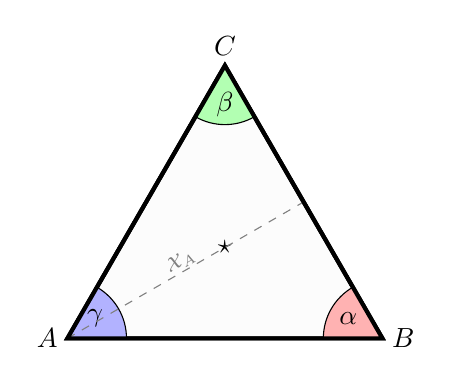
\begin{tikzpicture}
    % draw the background
    \draw [line width=1.5pt, fill=gray!2] (0,0) -- (60:4) -- (4,0) -- cycle;

    \coordinate[label=left:$A$]  (A) at (0,0);
    \coordinate[label=right:$B$] (B) at (4,0);
    \coordinate[label=above:$C$] (C) at (2,3.464);
    \coordinate[label=above:$\star$] (D) at (2,0.953);

%    \coordinate[label=below:$c$](c) at ($ (A)!.5!(B) $);
%    \coordinate[label=left:$b$](b) at ($ (A)!.5!(C) $);
%    \coordinate[label=right:$a$](a) at ($ (B)!.5!(C) $);

    % angle alpha
    \draw[fill=blue!30] (0,0) -- (0:0.75cm) arc (0:60:.75cm);
    \draw (0.35cm,0.25cm) node {$\gamma$};

    % angle beta
    \begin{scope}[shift={(4cm,0cm)}]
        \draw[fill=red!30] (0,0) -- (-180:0.75cm) arc (180:120:0.75cm);
%        \draw[color=gray, dashed] (0,0) -- node[sloped, above=-0.1cm] {$\scriptstyle h_b$} (150:3.464cm);
        \draw (150:0.5cm) node {$\alpha$};
    \end{scope}

    % angle gamma
    \begin{scope}[shift={(60:4)}]
        \draw[fill=green!30] (0,0) -- (-120:.75cm) arc (-120:-60:.75cm);
%        \draw[color=gray, dashed] (0,0) -- node[right=-0.1cm] {$\scriptstyle h_c$} (-90:3.464cm);
        \draw (-90:0.5cm) node {$\beta$};
    \end{scope}

% Sign for right angle of h_c
%    \begin{scope}[shift={(2,0)}]
%        \draw[fill=gray!30] (0,0) -- node[above=-0.15cm,near start] {$\cdot$} (0:0.18cm)
%                           arc (0:90:.18cm);
%    \end{scope}

% sign of right angle of h_a
%    \begin{scope}[shift={(30:3.464cm)}]
%        \draw[fill=gray!30] (0,0) -- node[near end,right=-0.28cm] {$\cdot$} (-60:0.18cm)
%                            arc (-60:-150:.18cm);
%    \end{scope}

% sign of right angle of h_b
%    \begin{scope}[shift={(60:2cm)}]
%        \draw[fill=gray!30] (0,0) -- node[right=-0.08cm, near start] {$\cdot$} (60:0.18cm)
%                            arc (60:-30:.18cm);
%    \end{scope}

    % Height with label
    \draw[color=gray, dashed] (0,0) -- node[sloped, above=-0.1cm] {$\scriptstyle \mathcal{X}_{A}$} (30:3.464cm);

    % The triangle
    \draw [line width=1.5pt] (0,0) -- (60:4) -- (4,0) -- cycle;
  \end{tikzpicture}

%  
% Reflexi�n A  
%
  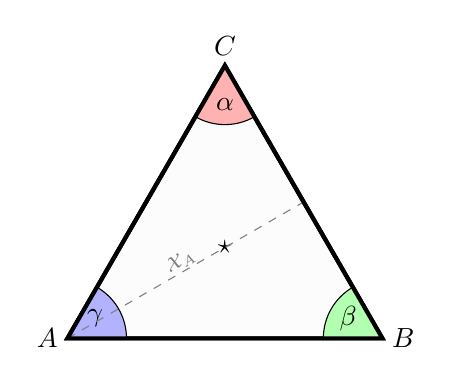
\begin{tikzpicture}
    % draw the background
    \draw [line width=1.5pt, fill=gray!2] (0,0) -- (60:4) -- (4,0) -- cycle;

    \coordinate[label=left:$A$]  (A) at (0,0);
    \coordinate[label=right:$B$] (B) at (4,0);
    \coordinate[label=above:$C$] (C) at (2,3.464);
    \coordinate[label=above:$\star$] (D) at (2,0.953);

%    \coordinate[label=below:$c$](c) at ($ (A)!.5!(B) $);
%    \coordinate[label=left:$b$](b) at ($ (A)!.5!(C) $);
%    \coordinate[label=right:$a$](a) at ($ (B)!.5!(C) $);

    % angle alpha
    \draw[fill=blue!30] (0,0) -- (0:0.75cm) arc (0:60:.75cm);
    \draw (0.35cm,0.25cm) node {$\gamma$};

    % angle beta
    \begin{scope}[shift={(4cm,0cm)}]
        \draw[fill=green!30] (0,0) -- (-180:0.75cm) arc (180:120:0.75cm);
%        \draw[color=gray, dashed] (0,0) -- node[sloped, above=-0.1cm] {$\scriptstyle h_b$} (150:3.464cm);
        \draw (150:0.5cm) node {$\beta$};
    \end{scope}

    % angle gamma
    \begin{scope}[shift={(60:4)}]
        \draw[fill=red!30] (0,0) -- (-120:.75cm) arc (-120:-60:.75cm);
%        \draw[color=gray, dashed] (0,0) -- node[right=-0.1cm] {$\scriptstyle h_c$} (-90:3.464cm);
        \draw (-90:0.5cm) node {$\alpha$};
    \end{scope}

% Sign for right angle of h_c
%    \begin{scope}[shift={(2,0)}]
%        \draw[fill=gray!30] (0,0) -- node[above=-0.15cm,near start] {$\cdot$} (0:0.18cm)
%                           arc (0:90:.18cm);
%    \end{scope}

% sign of right angle of h_a
%    \begin{scope}[shift={(30:3.464cm)}]
%        \draw[fill=gray!30] (0,0) -- node[near end,right=-0.28cm] {$\cdot$} (-60:0.18cm)
%                            arc (-60:-150:.18cm);
%    \end{scope}

% sign of right angle of h_b
%    \begin{scope}[shift={(60:2cm)}]
%        \draw[fill=gray!30] (0,0) -- node[right=-0.08cm, near start] {$\cdot$} (60:0.18cm)
%                            arc (60:-30:.18cm);
%    \end{scope}

    % Height with label
    \draw[color=gray, dashed] (0,0) -- node[sloped, above=-0.1cm] {$\scriptstyle \mathcal{X}_{A}$} (30:3.464cm);

    % The triangle
    \draw [line width=1.5pt] (0,0) -- (60:4) -- (4,0) -- cycle;
  \end{tikzpicture}     
\end{document}